\documentclass[10pt]{beamer}
\usepackage{lmodern}
\usepackage[utf8]{vietnam}
\usepackage{amsmath}
\usepackage{listings}
\usepackage{xcolor}
\usefonttheme{structurebold}
\usetheme{Rochester}

\usepackage[backend=biber]{biblatex}

\definecolor{codegreen}{rgb}{0,0.6,0}
\definecolor{codegray}{rgb}{0.5,0.5,0.5}
\definecolor{codepurple}{rgb}{0.58,0,0.82}
\definecolor{backcolour}{rgb}{0.95,0.95,0.92}

\lstdefinestyle{mystyle}{
    backgroundcolor=\color{backcolour},   
    commentstyle=\color{codegreen},
    keywordstyle=\color{magenta},
    numberstyle=\tiny\color{codegray},
    stringstyle=\color{codepurple},
    basicstyle=\ttfamily\footnotesize,
    breakatwhitespace=false,         
    breaklines=true,                 
    captionpos=b,                    
    keepspaces=true,                 
    numbers=left,                    
    numbersep=5pt,                  
    showspaces=false,                
    showstringspaces=false,
    showtabs=false,                  
    tabsize=2
}

\lstset{style=mystyle}


\addbibresource{presentation.bib}

\setbeamertemplate{navigation symbols}{\insertlogo}

\begin{document}
\author{Thu-Ngan Doan, Hoang-Quan Tran, Tan-Tho Huynh, Nhat-Dang Su, Diem-Uyen Phan-Dang}
\title{Efficiency of the Simplex Method}
\subtitle{Investigating on how fast Simplex Method will solve a problem in a given size.}
\logo{
\includegraphics[scale=.2]{img/fithcmuslogo.png}}
\institute{VNUHCM - University of Science}
\date{Spring 2022}
\subject{CSC10104 - Linear Programming}

\setbeamercovered{transparent}
\setbeamertemplate{navigation symbols}{}

\begin{frame}[plain]
\maketitle
\end{frame}

\begin{frame}
\frametitle{Mục lục}
\tableofcontents
\end{frame}

\section{Giới thiệu}
\begin{frame}{Giới thiệu}

\end{frame}

\section{Performance Measures}
\begin{frame}{Performance Measures}
Can be divied into two types:
\begin{itemize}
\item Worst case: asking how much efforts is needed to solve all problems of a given \textit{size}
\item Average case: looking at the average amount of effort, averaging over all problems of a giving \textit{size}. 
\end{itemize}
Worst-case analyses are generally easier than Average-case.
\end{frame}

\section{Measuring the Size of a Problem}
\begin{frame}{Measuring the Size of a Problem}

\end{frame}

\section{Measuring the Effort to Solve a Problem}
\begin{frame}{Measuring the Effort to Solve a Problem}

\end{frame}

\section{Worst-case Analysis of the Simplex Method}
\begin{frame}{Worst-case Analysis of the Simplex Method}
\begin{itemize}
\item Số phương án chấp nhận được tối đa có thể chọn là $\displaystyle \binom{n + m}{n}$.
\item Trong trường hợp xấu nhất, $n + m$ đạt giá trị lớn nhất khi $m = n$.
\item Ta có thể ước lượng một chặn trên và chặn dưới của $\displaystyle \binom{2n}{n}$\cite{Vanderbei2020}:
$$
\frac{2^{2n}}{2n} \leq \binom{2n}{n} \leq 2^{2n} \ (n \in \mathbb{N^+})
$$
\end{itemize}
\end{frame}
\begin{frame}{Worst-case Analysis of the Simplex Method (cont.) - Proof}
\begin{theorem}[Xấp xỉ Stirling\cite{weisstein}]
$$
\displaystyle
n! \operatorname*{\sim}_{n\to\infty} \sqrt{2\pi n}\left(\frac{n}{e}\right)^n
$$
\end{theorem}
Khai triển $\displaystyle \binom{2n}{n} = \frac{(2n)!}{(n!)^2}$\footnote{$\binom{n}{k} = \frac{n!}{(n - k)!k!}$}. Ta cũng có các xấp xỉ sau:
\begin{itemize}
\item $\displaystyle (2n)! \operatorname*{\sim}_{n\to\infty} 2\sqrt{\pi n} \left(\frac{2n}{e}\right)^{2n}$ 
\item $\displaystyle (n!)^2 \operatorname*{\sim}_{n\to\infty} 2\pi n \left(\frac{n}{e}\right)^{2n}$ 
\end{itemize}
Qua đó, $\displaystyle \binom{2n}{n} \operatorname*{\sim}_{n\to\infty} \frac{2\sqrt{\pi n} \left(\frac{2n}{e}\right)^{2n}}{2\pi n \left(\frac{n}{e}\right)^{2n}} =  \frac{2^{2n}}{\sqrt{\pi n}}$
\end{frame}

\begin{frame}{Worst-case Analysis of the Simplex Method (cont.) - Proof}
\begin{proof}
Gọi
$$
\displaystyle
L = \frac{\frac{2^{2n}}{2n}}{\frac{2^{2n}}{\sqrt{\pi n}}} = \frac{2^{2n}\sqrt{\pi n}}{2^{2n} 2n} = \frac{\sqrt{\pi}}{2\sqrt{n}} < 1,\ \forall n \in \mathbb{N^+}
$$
Do $L < 1$, ta có thể kết luận $\frac{2^{2n}}{2n} \leq \frac{2^{2n}}{\sqrt{\pi n}},\ \forall n \in \mathbb{N^+}
$. Khi đó
$$
\displaystyle
\frac{2^{2n}}{2n} \leq \frac{2^{2n}}{\sqrt{\pi n}} \leq 2^{2n} \iff \frac{2^{2n}}{2n} \leq \binom{2n}{n} \leq 2^{2n}
$$
\end{proof}
Trong trường hợp xấu nhất, thuật toán có độ phức tạp thuộc nhóm $\mathcal{O}(2^{2n})$. $2^{2n}$ \textbf{rất lớn} dù $n$ không lớn lắm. (e.g $n = 25$, $2^{50} = 1.1259\times 10^{15}$)
\end{frame}

\begin{frame}{Worst-case Analysis of the Simplex Method (cont.) - Example}
Năm 1972, V. Klee and G.J. Minty\cite{klee1970good} đề xuất bài toán Minty-Klee, theo đó phương pháp đơn hình cần ít nhất $2^n - 1$ lần lặp để giải:
\begin{equation*}
\sum_{j = 1}^{n} 2^{n - j} x_j \rightarrow \max
\end{equation*}
các ràng buộc
\begin{equation*}
\begin{aligned}
2\sum_{j = 1}^{i - 1} 2^{i - j}x_j + x_i &\leq 100^{i - 1} & (i = 1, 2, .., n)\\
x_j &\geq 0 & (j = 1, 2, .., n)
\end{aligned}
\end{equation*}
Theo đó 3 ràng buộc đầu tiên
$$
\left\{
\begin{array}{lll}
x_1 &\leq 1\\
4x_1 + x_2 &\leq 10^2\\
8x_1 + 4x_2 + x_3 &\leq 10^4
\end{array}
\right.
$$
\end{frame}

\begin{frame}{Worst-case Analysis of the Simplex Method (cont.) - Example}
Dễ thấy đây chỉ là tập các cận trên của mỗi biến:
$$
\begin{array}{lll}
0 \leq x_1 &\leq 1\\
0 \leq x_2 &\leq 10^2\\
0 \leq x_3 &\leq 10^4
\end{array}
$$
Do đó, tập các ràng buộc trở thành tập các cận trên, biến miền ràng buộc trên không gian $n$ chiều thành một siêu lập phương:
$$
\begin{array}{lll}
0 \leq x_1 &\leq 1\\
0 \leq x_2 &\leq 100\\
&\vdots\\
0 \leq x_n &\leq 100^{n - 1}
\end{array}
$$
\end{frame}

\begin{frame}{Worst-case Analysis of the Simplex Method (cont.) - Example}
Miền chấp thuận của bài toán Klee-Minty còn được gọi là Siêu lập phương\footnote{Siêu lập phương $n$ chiều có $2^n$ đỉnh\cite{10945-3852}} Klee-Minty.
\begin{figure}
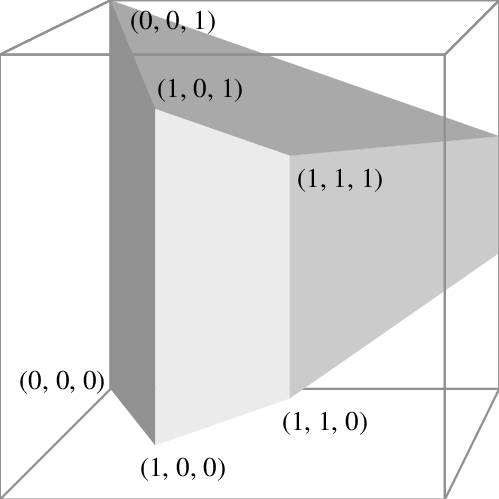
\includegraphics[scale=.15]{img/klee-minty-cube.png}
\caption{Ví dụ cho Siêu lập phương Klee-Minty với $n = 3$ và $\epsilon = \frac{1}{3}$}
\end{figure}
Phương pháp đơn hình sẽ xuất phát từ 1 đỉnh, đi qua tất cả các đỉnh trước khi tìm ra phương án tối ưu.
\end{frame}

\begin{frame}{Worst-case Analysis of the Simplex Method (cont.) - Example}
Đặt $\beta_i = 100^{i - 1}$. Bài toán Minty-Klee có dạng tổng quát:
$$
\sum_{j = 1}^n 2^{n - j}x_j - \frac{1}{2}\sum_{j = 1}^n 2^{n - j}\beta_j \rightarrow \max
$$
các ràng buộc
$$
\begin{aligned}
2\sum_{j = 1}^{i - 1} 2^{i - j}x_j + x_i &\leq \sum_{j = 1}^{i - 1}2^{i - j}\beta_j + \beta_i\ &(i = 1, 2, .., n)\\
x_j &\geq 0 &(j = 1, 2, .., n)
\end{aligned}
$$
\end{frame}

\begin{frame}{Worst-case Analysis of the Simplex Method (cont.) - Example}
Với $n = 3$, bài toán được phát biểu như sau:
$$
4x_1 + 2x_2 + x_3 - 2\beta_1 - \beta_2 - \frac{1}{2}\beta_3 \rightarrow \max
$$
Các ràng buộc:
$$
\left\{
\begin{array}{lll}
x_1 &\leq \beta_1\\
4x_1 + x_2 &\leq 2\beta_1 + \beta_2\\
8x_1 + 4x_2 + x_3 &\leq 4\beta_1 + 2\beta_2 + \beta_3
\end{array}
\right.
$$
Ta thêm biến để được các đẳng thức:
$$
\left\{
\begin{array}{lll}
x_1 & + \ x_4 & = \beta_1\\
4x_1 + x_2 & + \ x_5 & = 2\beta_1 + \beta_2\\
8x_1 + 4x_2 + x_3 & + \ x_6 & = 4\beta_1 + 2\beta_2 + \beta_3\\
x_4, \ x_5, \ x_6 & &\geq 0
\end{array}
\right.
$$
Cơ sở: $(x_4, x_5, x_6)$
\end{frame}

\begin{frame}{Worst-case Analysis of the Simplex Method (cont.) - Example}
Bảng đơn hình xuất phát:
\begin{table}[H]
\centering
\begin{tabular}{|c|c|c|c|c|c|c|c|c|}
\hline
CS & HS & PA & 4 & 2 & 1 & 0 & 0 & 0 \\
\hline
$x_4$ & 0 & $\beta_1$ & 1 & 0 & 0 & 1 & 0 & 0 \\
$x_5$ & 0 & $2\beta_1 + \beta_2$ & 4 & 1 & 0 & 0 & 1 & 0 \\
$x_6$ & 0 & $4\beta_1 + 2\beta_2 + \beta_3$ & 8 & 4 & 1 & 0 & 0 & 1 \\
\hline
\multicolumn{2}{|c|}{max}
& 0 & -4 & -2 & -1 & 0 & 0 & 0 \\
\hline
\end{tabular}
\end{table}
\begin{itemize}
\item Tồn tại 3 cột ứng với $\Delta < 0$, ta chọn cột có $\Delta = -4$  
\item So sánh: $\dfrac{\beta_1}{1} < \dfrac{2\beta_1 + \beta_2}{4} < \dfrac{4\beta_1 + 2\beta_2 + \beta_3}{8}$ nên ta chọn dòng 1  
\item $x_4$ ra, $x_1$ vào
\end{itemize}
\end{frame}

\begin{frame}{Worst-case Analysis of the Simplex Method (cont.) - Example}
Lần lặp thứ 1:
\begin{table}[H]
\centering
\begin{tabular}{|c|c|c|c|c|c|c|c|c|}
\hline
CS & HS & PA & 4 & 2 & 1 & 0 & 0 & 0 \\
\hline
$x_1$ & 4 & $\beta_1$ & 1 & 0 & 0 & 1 & 0 & 0 \\
$x_5$ & 0 & $-2\beta_1 + \beta_2$ & 0 & 1 & 0 & -4 & 1 & 0 \\
$x_6$ & 0 & $-4\beta_1 + 2\beta_2 + \beta_3$ & 0 & 4 & 1 & -8 & 0 & 1 \\
\hline
\multicolumn{2}{|c|}{max}
& $4\beta_1$ & 0 & -2 & -1 & 4 & 0 & 0 \\
\hline
\end{tabular}
\end{table}
\begin{itemize}
\item Tồn tại 2 cột ứng với $\Delta < 0$, ta chọn cột có $\Delta = -2$
\item So sánh: $\dfrac{-2\beta_1 + \beta_2}{1} < \dfrac{-4\beta_1 + 2\beta_2 + \beta_3}{4}$ nên ta chọn dòng 2
\item $x_5$ ra, $x_2$ vào
\end{itemize}
\end{frame}

\begin{frame}{Worst-case Analysis of the Simplex Method (cont.) - Example}
Lần lặp thứ 2:
\begin{table}[H]
\centering
\begin{tabular}{|c|c|c|c|c|c|c|c|c|}
\hline
CS & HS & PA & 4 & 2 & 1 & 0 & 0 & 0 \\
\hline
$x_1$ & 4 & $\beta_1$ & 1 & 0 & 0 & 1 & 0 & 0 \\
$x_2$ & 2 & $-2\beta_1 + \beta_2$ & 0 & 1 & 0 & -4 & 1 & 0 \\
$x_6$ & 0 & $4\beta_1 - 2\beta_2 + \beta_3$ & 0 & 0 & 1 & 8 & -4 & 1 \\
\hline
\multicolumn{2}{|c|}{max}
& $2\beta_2$ & 0 & 0 & -1 & -4 & 2 & 0 \\
\hline
\end{tabular}
\end{table}
\begin{itemize}
\item Tồn tại 2 cột ứng với $\Delta < 0$, ta chọn cột có $\Delta = -4$
\item So sánh: $\dfrac{\beta_1}{1} < \dfrac{4\beta_1 - 2\beta_2 + \beta_3}{8}$ nên ta chọn dòng 1
\item $x_1$ ra, $x_4$ vào
\end{itemize}
\end{frame}

\begin{frame}{Worst-case Analysis of the Simplex Method (cont.) - Example}
Lần lặp thứ 3:
\begin{table}[H]
\centering
\begin{tabular}{|c|c|c|c|c|c|c|c|c|}
\hline
CS & HS & PA & 4 & 2 & 1 & 0 & 0 & 0 \\
\hline
$x_4$ & 0 & $\beta_1$ & 1 & 0 & 0 & 1 & 0 & 0 \\
$x_2$ & 2 & $2\beta_1 + \beta_2$ & 4 & 1 & 0 & 0 & 1 & 0 \\
$x_6$ & 0 & $-4\beta_1 - 2\beta_2 + \beta_3$ & -8 & 0 & 1 & 0 & -4 & 1 \\
\hline
\multicolumn{2}{|c|}{max}
& $4\beta_1 + 2\beta_2$ & 4 & 0 & -1 & 0 & 2 & 0 \\
\hline
\end{tabular}
\end{table}
\begin{itemize}
\item Tồn tại 1 cột ứng với $\Delta < 0$, ta chọn cột $\Delta = -1$
\item $x_6$ ra, $x_3$ vào
\end{itemize}
\end{frame}

\begin{frame}{Worst-case Analysis of the Simplex Method (cont.) - Example}
Lần lặp thứ 4:
\begin{table}[H]
\centering
\begin{tabular}{|c|c|c|c|c|c|c|c|c|}
\hline
CS & HS & PA & 4 & 2 & 1 & 0 & 0 & 0 \\
\hline
$x_4$ & 0 & $\beta_1$ & 1 & 0 & 0 & 1 & 0 & 0 \\
$x_2$ & 2 & $2\beta_1 + \beta_2$ & 4 & 1 & 0 & 0 & 1 & 0 \\
$x_3$ & 1 & $-4\beta_1 - 2\beta_2 + \beta_3$ & -8 & 0 & 1 & 0 & -4 & 1 \\
\hline
\multicolumn{2}{|c|}{max}
& $\beta_3$ & -4 & 0 & 0 & 0 & -2 & 1 \\
\hline
\end{tabular}
\end{table}
\begin{itemize}
\item Tồn tại 2 cột ứng với $\Delta < 0$, ta chọn cột $\Delta = -4$
\item So sánh: $\dfrac{\beta_1}{1} < \dfrac{2\beta_1 + \beta_2}{4}$ nên ta chọn dòng 1
\item $x_4$ ra, $x_1$ vào
\end{itemize}
\end{frame}

\begin{frame}{Worst-case Analysis of the Simplex Method (cont.) - Example}
Lần lặp thứ 5
\begin{table}[H]
\centering
\begin{tabular}{|c|c|c|c|c|c|c|c|c|}
\hline
CS & HS & PA & 4 & 2 & 1 & 0 & 0 & 0 \\
\hline
$x_1$ & 4 & $\beta_1$ & 1 & 0 & 0 & 1 & 0 & 0 \\
$x_2$ & 2 & $-2\beta_1 + \beta_2$ & 0 & 1 & 0 & -4 & 1 & 0 \\
$x_3$ & 1 & $4\beta_1 - 2\beta_2 + \beta_3$ & 0 & 0 & 1 & 8 & -4 & 1 \\
\hline
\multicolumn{2}{|c|}{max}
& $4\beta_1 + \beta_3$ & 0 & 0 & 0 & 4 & -2 & 1 \\
\hline
\end{tabular}
\end{table}
\begin{itemize}
\item Tồn tại 1 cột ứng với $\Delta < 0$, ta chọn cột $\Delta = -2$
\item $x_2$ ra, $x_5$ vào
\end{itemize}
\end{frame}

\begin{frame}{Worst-case Analysis of the Simplex Method (cont.) - Example}
Lần lặp thứ 6
\begin{table}[H]
\centering
\begin{tabular}{|c|c|c|c|c|c|c|c|c|}
\hline
CS & HS & PA & 4 & 2 & 1 & 0 & 0 & 0 \\
\hline
$x_1$ & 4 & $\beta_1$ & 1 & 0 & 0 & 1 & 0 & 0 \\
$x_5$ & 0 & $-2\beta_1 + \beta_2$ & 0 & 1 & 0 & -4 & 1 & 0 \\
$x_3$ & 1 & $-4\beta_1 + 2\beta_2 + \beta_3$ & 0 & 4 & 1 & -8 & 0 & 1 \\
\hline
\multicolumn{2}{|c|}{max}
& $2\beta_2 + \beta_3$ & 0 & 2 & 0 & -4 & 0 & 1 \\
\hline
\end{tabular}
\end{table}
\begin{itemize}
\item Tồn tại 1 cột ứng với $\Delta < 0$, ta chọn cột $\Delta = -4$
\item $x_1$ ra, $x_4$ vào
\end{itemize}
\end{frame}


\begin{frame}{Worst-case Analysis of the Simplex Method (cont.) - Example}
Lần lặp thứ 7
\begin{table}[H]
\centering
\begin{tabular}{|c|c|c|c|c|c|c|c|c|}
\hline
CS & HS & PA & 4 & 2 & 1 & 0 & 0 & 0 \\
\hline
$x_4$ & 0 & $\beta_1$ & 1 & 0 & 0 & 1 & 0 & 0 \\
$x_5$ & 0 & $2\beta_1 + \beta_2$ & 4 & 1 & 0 & 0 & 1 & 0 \\
$x_3$ & 1 & $4\beta_1 + 2\beta_2 + \beta_3$ & 8 & 4 & 1 & 0 & 0 & 1 \\
\hline
\multicolumn{2}{|c|}{max}
&  $4\beta_1 + 2\beta_2 + \beta_3$  & 4 & 2 & 0 & 0 & 0 & 1 \\
\hline
\end{tabular}
\end{table}
Tất cả $\Delta \ge 0$, bài toán tìm được phương án tối ưu.
\end{frame}


\section{Empirical Average Performance of the Simplex Method}
\begin{frame}{Empirical Average Performance of the Simplex Method - Thiết lập bài toán}
Giả sử ta có một bài toán quy hoạch tuyến tính với n biến và m ràng buộc. Ta gọi:
\begin{itemize}
\item A là ma trận $m\times n$ chứa các hệ số của hệ ràng buộc
\item b là ma trận $m\times 1$ chứa các giá trị bên vế phải của hệ ràng buộc
\item c là ma trận $1\times n$ chứa các hệ số của hàm mục tiêu
\end{itemize}
\end{frame}

\begin{frame}[fragile]{Empirical Average Performance of the Simplex Method (cont.) - Thiết lập bài toán}
Ta phát sinh ngẫu nhiên một bài toán quy hoạch tuyến tính
\begin{lstlisting}[language=Matlab]
m = round(10*exp(log(100)*rand()));
n = round(10*exp(log(100)*rand()));
sigma = 10;
A = round(sigma*(randn(m,n)));
b = round(sigma*abs(randn(m,1)));
c = round(sigma*randn(1,n));
\end{lstlisting}
\end{frame}

\begin{frame}[fragile]{Empirical Average Performance of the Simplex Method (cont.) - Thiết lập bài toán}
Tại mỗi lần lặp, ta chọn \textbf{biến vào} là biến có hệ số lớn nhất trong hàm mục tiêu
\begin{lstlisting}[language=Matlab]
iter = 0;
while max(c) > eps
    [cj, col] = max(c);
    Acol = A(:,col);
    if sum(Acol < -eps) == 0
        opt = -1;
        'unbounded'
        break;
    end
\end{lstlisting}
\end{frame}

\begin{frame}[fragile]{Empirical Average Performance of the Simplex Method (cont.) - Thiết lập bài toán}
Tiếp theo, ta chọn \textbf{biến ra} là biến có tỉ số giữa $b_i$ và $a_{i_k}$ bé nhất
\begin{lstlisting}[language=Matlab]
    nums = b.*(Acol < -eps);
    dens = -Acol.*(Acol < -eps);
    [t, row] = min(nums./dens);
    Arow = A(row,:);
    a = A(row,col);
\end{lstlisting}
Ta có được phần tử xoay
\end{frame}

\begin{frame}[fragile]{Empirical Average Performance of the Simplex Method (cont.) - Thiết lập bài toán}
Cuối cùng, ta cập nhật các hệ số trong hàm mục tiêu, các phương án, và các hệ số ràng buộc
\begin{lstlisting}[language=Matlab]
    A = A - Acol*Arow/a;
    A(row,:) = -Arow/a;
    A(:,col) = Acol/a;
    A(row,col) = 1/a;
    
    brow = b(row);
    b = b - brow*Acol/a;
    b(row) = -brow/a;
    
    ccol = c(col);
    c = c - ccol*Arow/a;
    c(col) = ccol/a;
    
    iter = iter + 1;
end
\end{lstlisting}
\end{frame}

\begin{frame}[fragile]{Empirical Average Performance of the Simplex Method (cont.) - Kết quả thực nghiệm}
\begin{figure}
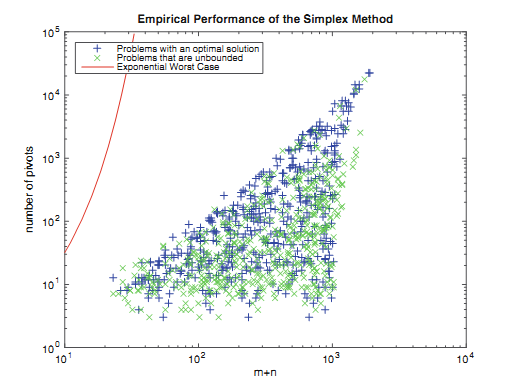
\includegraphics[scale=.5]{img/plot_1.png}
\caption{Đồ thị log-log thể hiện mối tương quan giữa $m$ + $n$ và số điểm xoay của bảng đơn hình (sample size = 1000)}
\end{figure}
\end{frame}

\begin{frame}[fragile]{Empirical Average Performance of the Simplex Method (cont.) - Kết quả thực nghiệm}
Dựa vào đồ thị, ta có được thông tin: \\
\textcolor{red}{- Đồ thị trên là đồ thị log-log, nên đừng vội kết luận rằng số điểm xoay tăng xấp xỉ tuyến tính so với $n$ + $m$} \\
- Trong 1000 mẫu dữ liệu: có 501 mẫu trong dữ liệu có phương án tối ưu, trong khi 499 mẫu còn lại thì không có \\
- Số lượng bài toán có $m$ > $n$ và $m$ < $n$ là xấp xỉ bằng nhau \\
- Những bài toán có $m$ > $n$ gần như luôn có phương án tối ưu, và theo chiều ngược lại, $n$ < $m$ lại cho ta những bài toán nhiều khả năng là không có\\
\end{frame}

\section{References}
\begin{frame}[allowframebreaks]{References}
\printbibliography
\end{frame}
\end{document}
